\chapter{Graph Operations}

Rishnak found Ajur walking with Jura. Not wasting a moment, Rishnak started the session. He said, ``Today we will discuss various graph operations.''

Eager to learn, Ajur asked, ``Are they similar to arithmetic operations like addition, subtraction, and multiplication that operate on numbers? Or set operations such as union, intersection, and complement?''

Rishnak said, ``There are many binary operations\footnote{Here, binary means operating on two operands.} and since graphs are represented as sets, many of the operations are similar to set operations. Each graph operation typically generates another graph. We can also see how graphs evolve. Let us walk through a few of these operations.''

Rishnak described the following binary graph operations, flashing his hands to form figures as he went on:
\begin{enumerate}
    \item \textit{Graph union:} Let graph~$G_3=(V_3,E_3)$ denote the union of two graphs~$G_1=(V_1,E_1)$ and~$G_2=(V_2,E_2)$. Then $V_3=V_1\cup V_2$ and~$E_3=E_1\cup E_2$. Naturally, graph~$G_3$ is not connected.
    \item \textit{Graph complement:} The complement of graph~$G=(V_1,E_1)$ [Figure~\ref{17g1}] is Graph~$H=(V_2,E_2)$ [Figure~\ref{17g2}] if~$V_2=V_1$ and $E_2=\{e|e\notin E_1\}$.
    \item \textit{Vertex addition:} Vertex addition applied to graph~$G_1=(V_1,E_1)$ [Figure~\ref{17g1}] produces graph~$G_2=(V_2,E_2)$ [Figure~\ref{17g3}], where $V_2=V_1\cup\{x|x\notin V_1\}$ and~$E_2=E_1\cup\{(x,y)|x\in V_2\ \text{and}\ y\in Y\subset V_1\}$.\footnote{Barabassi-Albert used a version of this to generate graphs. In the Barabassi-Albert model, the new vertex adds an edge to an existing vertex with a probability related to the degree of that vertex to generate graphs.}
    \item  \textit{Cartesian product:} The Cartesian product~$G_1\square G_2$ is graph~$G_3$ such that the vertex set of $G_3$ is Cartesian product~$V(G_1)\times V(G_2)$ and two vertices~$(u,u')$ and $(v,v')$ are adjacent in~$G_3$ if and only if either~$u=v$ and~$u'$ is adjacent to~$v'$ in~$G_2$ or~$u'=v'$ and~$u$ is adjacent to~$v$ in~$G_1$. [Figure~\ref{17g4}] [Figure~\ref{17g5}] [Figure~\ref{17g6}]
    \item \textit{Line graph:} Given graph~$G$, the line graph of~$G$, denoted by~$L(G)$, is a graph with each vertex of~$L(G)$ representing an edge of~$G$ and two vertices in~$L(G)$ being adjacent if the corresponding edges share a common end vertex. [Figure~\ref{17g7}] [Figure~\ref{17g8}]
\end{enumerate}

\begin{figure}
\begin{center}
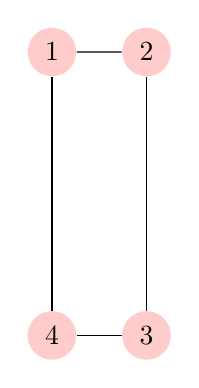
\begin{tikzpicture}
  [scale=.6,auto=left,every node/.style={circle,fill=red!20}]
  \node (n1) at (1,7) {1};
  \node (n2) at (3,7)  {2};
  \node (n4) at (1,1)  {4};
  \node (n3) at (3,1)  {3};

  \foreach \from/\to in {n1/n2,n2/n3,n3/n4,n1/n4}
    \draw (\from) -- (\to);

\end{tikzpicture}
\caption{Example graph for which we wish to apply the union and complement operations, as well as vertex addition}\label{17g1}
\end{center}
\end{figure}

\begin{figure}
\begin{center}
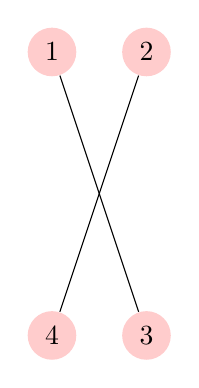
\begin{tikzpicture}
  [scale=.6,auto=left,every node/.style={circle,fill=red!20}]
  \node (n1) at (1,7) {1};
  \node (n2) at (3,7)  {2};
  \node (n4) at (1,1)  {4};
  \node (n3) at (3,1)  {3};

  \foreach \from/\to in {n1/n3,n2/n4}
    \draw (\from) -- (\to);

\end{tikzpicture}
\caption{Complement of the graph shown in Figure~\ref{17g1}}\label{17g2}
\end{center}
\end{figure}
\begin{figure}
\begin{center}
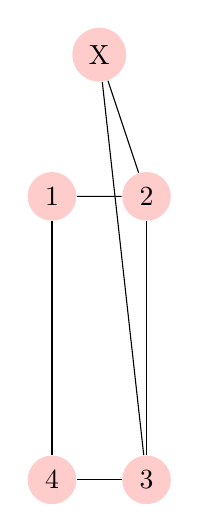
\begin{tikzpicture}
  [scale=.6,auto=left,every node/.style={circle,fill=red!20}]
  \node (n1) at (1,7) {1};
  \node (n2) at (3,7)  {2};
  \node (n4) at (1,1)  {4};
  \node (n3) at (3,1)  {3};
  \node (n5) at (2,10) {X};
  \foreach \from/\to in {n1/n2,n2/n3,n3/n4,n1/n4,n3/n5,n2/n5}
    \draw (\from) -- (\to);

\end{tikzpicture}
\caption{Adding a vertex and edges from that vertex to some subset of vertices in the graph shown in Figure~\ref{17g1}}\label{17g3}
\end{center}
\end{figure}

\begin{figure}
\begin{center}
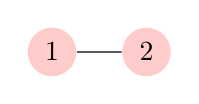
\begin{tikzpicture}
  [scale=.6,auto=left,every node/.style={circle,fill=red!20}]
  \node (n1) at (1,7) {1};
  \node (n2) at (3,7)  {2};

  \foreach \from/\to in {n1/n2}
    \draw (\from) -- (\to);

\end{tikzpicture}
\caption{Example graph~$G_1$ for which we wish to apply the Cartesian product}\label{17g4}
\end{center}
\end{figure}

\begin{figure}
\begin{center}
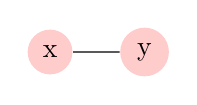
\begin{tikzpicture}
  [scale=.6,auto=left,every node/.style={circle,fill=red!20}]
  \node (n1) at (1,7) {x};
  \node (n2) at (3,7)  {y};

  \foreach \from/\to in {n1/n2}
    \draw (\from) -- (\to);

\end{tikzpicture}
\caption{Example graph~$G_2$ for which we wish to apply the Cartesian product}\label{17g5}
\end{center}
\end{figure}

\begin{figure}
\begin{center}
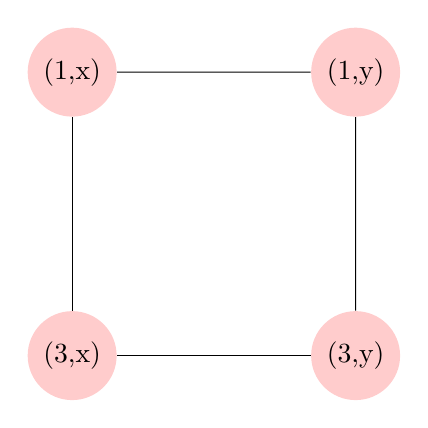
\begin{tikzpicture}
  [scale=.6,auto=left,every node/.style={circle,fill=red!20}]
  \node (n1) at (1,7) {(1,x)};
  \node (n2) at (7,7)  {(1,y)};
   \node (n3) at (1,1) {(3,x)};
   \node (n4) at (7,1) {(3,y)};
   
  \foreach \from/\to in {n1/n2,n1/n3,n2/n4,n3/n4}
    \draw (\from) -- (\to);

\end{tikzpicture}
\caption{The Cartesian product~$G_3$ of graphs~$G_1$ [Figure~\ref{17g4}] and~$G_2$ [Figure~\ref{17g5}]}\label{17g6}
\end{center}
\end{figure}

\begin{figure}
\begin{center}

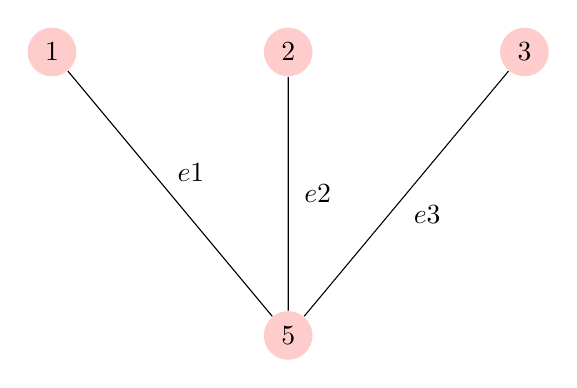
\begin{tikzpicture}
  [scale=.6,auto=left,every node/.style={circle,fill=red!20}]
  \tikzstyle{weight} = [fill=none]
  \node (n1) at (-1,5) {1};
  \node (n2) at (4,5)  {2};
  \node (n3) at (9,5)  {3};
  \node (n4) at (4,-1) {5};
 
\foreach \source /\dest /\weight in {n1/n4/e1,n2/n4/e2,n3/n4/e3} 
   \draw (\source) --node[weight] {$\weight$}  (\dest);
 
  \end{tikzpicture}
\caption{Example graph for which we wish to apply the line graph operation}\label {17g7}
\end{center}
\end{figure}

\begin{figure}
\begin{center}

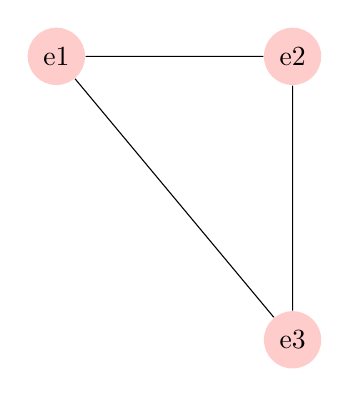
\begin{tikzpicture}
  [scale=.6,auto=left,every node/.style={circle,fill=red!20}]
  \tikzstyle{weight} = [draw=blue!5,shape=rectangle]
  \node (n1) at (-1,5) {e1};
  \node (n2) at (4,5)  {e2};
  \node (n3) at (4,-1) {e3};
 
\foreach \source /\dest  in {n1/n2,n2/n3,n3/n1} 
   \draw (\source) -- (\dest);
 
  \end{tikzpicture}
\caption {A line graph for the graph shown in Figure~\ref{17g7}}\label {17g8}
\end{center}
\end{figure}

\begin{figure}
\begin{center}
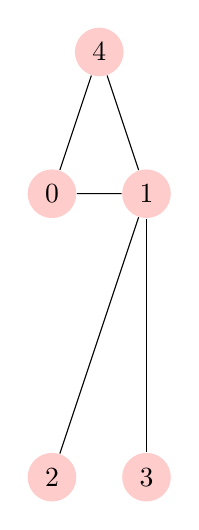
\begin{tikzpicture}
  [scale=.6,auto=left,every node/.style={circle,fill=red!20}]
  \node (n1) at (1,7) {0};
  \node (n2) at (3,7)  {1};
  \node (n4) at (1,1)  {2};
  \node (n3) at (3,1)  {3};
  \node (n5) at (2,10) {4};
  \foreach \from/\to in {n1/n5,n1/n2,n2/n5,n2/n4,n2/n3}
    \draw (\from) -- (\to);

\end{tikzpicture}
\caption{Randomly generated graph using the Erd\H{o}s--R\'enyi method with~$n=5$ vertices, $e=5$ edges, and edge probability~$0.5$}\label{17g9}
\end{center}
\end{figure}

Ajur listened intently at these graph operations, at times asking Rishnak to repeat the definition.

After some time, Rishnak said, ``The Petersen graph they we discussed before is actually the complement of the line graph of complete graph~$K_5$.''

Ajur tried to keep up. He knew that graph~$K_5$ was a complete graph with~10 edges. He also knew that the Petersen graph had~10 edges. Did they match? Ajur calculated that the line graph of~$K_5$ was a regular graph of degree~6 and therefore its complement would be a regular graph of degree~3, so that much matched. But still, he had to verify Rishnak's assertion in full, so he decided to work on it later.

Realizing that it was already getting late, Rishnak said, ``Let me also talk about graph construction. There is a method called the Erd\H{o}s--R\'enyi model\footnote{Named after mathematicians Paul Erd\H{o}s and Alfr\'ed R\'enyi.} for constructing graphs. In this method, for a graph with~$n$ vertices and~$e$ edges, for every unordered pair of vertices, an edge is present with the following probability:
$$\frac{e}{\frac{1}{2}n(n-1)}$$

Rishnak flashed his hands and a new graph appeared [Figure~\ref{17g9}]. He said, ``This graph is generated using the Erd\H{o}s--R\'enyi model with~$n=5$ and~$e=5$, so our edge probability is~$\frac{5}{10}=0.5$.\footnote{When Rishnak wrote this down later, he generated the graph using Sage Math (CoCALC) at \url{https://cocalc.com/}. You should try to generate a few graphs using this method.}

\subsection*{Question for the fifteenth day}
Rishnak said, ``For the question for the fifteenth day, can you draw the complement of the line graph of complete graph~$K_5$?''

\textit{Before you turn the page, try to come up with an answer of your own!}

\newpage
\subsection*{Answer for the fifteenth day}
Ajur remembered from earlier that he reasoned out that there would be~10 vertices in the line graph since~$K_5$ has~10 edges. He said, ``The complement will also have~10 vertices and will be a regular graph of degree~3 because the line graph will be a regular graph of degree~6.''

Ajur drew his answer in the dirt [Figure~\ref{15ga1}].

\begin{figure}
\begin{center}
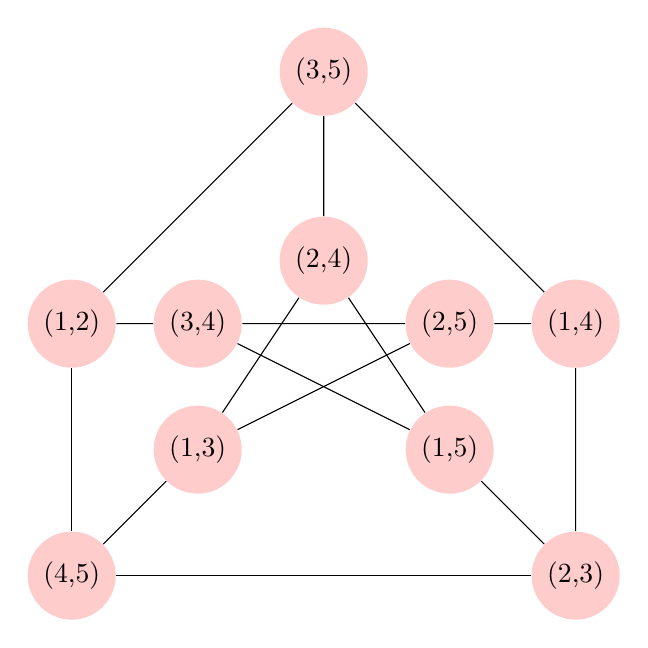
\begin{tikzpicture}
  [scale=.8,auto=left,every node/.style={circle,fill=red!20}]
  \node (n1) at (1,7) {(1,2)};
  \node (n2) at (5,11)  {(3,5)};
  \node (n3) at (9,7)  {(1,4)};
  \node (n4) at (9,3) {(2,3)};
  \node (n5) at (1,3) {(4,5)};
  \node (n6) at (3,7)  {(3,4)};
  \node (n7) at (5,8) {(2,4)};
  \node (n8)  at (7,7) {(2,5)};
  \node (n9) at (7,5) {(1,5)};
  \node (n10) at  (3,5) {(1,3)};
 
  \foreach \from/\to in {n1/n2,n2/n3,n3/n4,n4/n5,n5/n1,n1/n6,
  n2/n7, n3/n8, n4/n9, n5/n10, n6/n8, n8/n10, n10/n7,n7/n9,n9/n6}
    \draw (\from) -- (\to);


\end{tikzpicture}
\caption{The graph representing the complement of the line graph of complete graph~$K_5$; this graph is the Petersen graph}\label{15ga1}
\end{center}
\end{figure}

Ajur needed time to digest all of the new material from the day, so he and Jura drifted away as Rishnak proceeded to meet his other ghost friends.
